\section{Experiments}
\label{sec:results}

\subsection{Setup}
\label{ssec:setup}

Table~\ref{tab:simparams} lists the simulation parameters. All paired
evaluations use fixed run configurations and disjoint random seeds.
Monte-Carlo runs use the accelerated implementation validated by the
reference-comparison protocol of Claim~\ref{thm:initfaithful} and
Appendix~\ref{app:matlab}. Five experiments
are reported: 4-arm BER waterfall (\S\ref{ssec:exp1}), same-budget
classical heuristic (\S\ref{ssec:exp_omppk}), sampling-rate sensitivity
(\S\ref{ssec:exp_fs}), support recall and oracle-headroom probes
(\S\ref{ssec:exp_probes}), and complexity audit
(\S\ref{ssec:complexity_results}).

\begin{table}[t]
\centering
\caption{Simulation parameters. One configuration used for every receiver in every experiment.}
\label{tab:simparams}
\resizebox{\linewidth}{!}{%
\begin{tabular}{ll}
\toprule
\textbf{Parameter} & \textbf{Value} \\
\midrule
Sub-carriers $\Nsub$ & 1024 \\
Sub-carrier spacing $\Delta f$ & 15~Hz \\
Carrier $\fc$ & 12~kHz \\
Bandwidth $B$ & 4~kHz \\
Sampling rate $\fs$ & $4B=16$~kHz \\
Physical paths $\Ppath$ & 8 \\
Delay spread $\tau_{\text{spread}}$ & 10~ms (exp.\ PDP, $\tau_{\text{mean}}=0.8$~ms) \\
Per-path velocity $v$ & $\mathcal{N}(2,0.5^2)$~m/s \\
Dirichlet half-width $\kleak$ & 2 ($\Rightarrow$ 5 virtual taps / path) \\
Modulation & QPSK, Gray demapping \\
Pilot power fraction $\rhop$ & 0.5 \\
Pilot sequence & Zadoff--Chu root $r=7$, length $\Nsub$ \\
Outer iter.\ $T_\text{out}$ & 5 \\
MP-BP inner iter.\ $T_\text{mp}$ & 20 \\
OMP $(\lmax,\kmax,Q)$ at $\fs=4B$ & $(160,2,800)$ \\
\bottomrule
\end{tabular}
}
\end{table}

\subsection{4-arm BER waterfall and paired McNemar reductions}
\label{ssec:exp1}

Fig.~\ref{fig:ber4b} plots the paired-frame BER (left) and NMSE (right)
for the four receivers at $\fs=4B$, and Table~\ref{tab:ber4b} reports
the 3-seed pooled paired-BER reductions of the learned head relative to
the classical joint with paired McNemar $p$-values and Clopper--Pearson
95\% CIs at high SNR.

\begin{figure}[t]
\centering
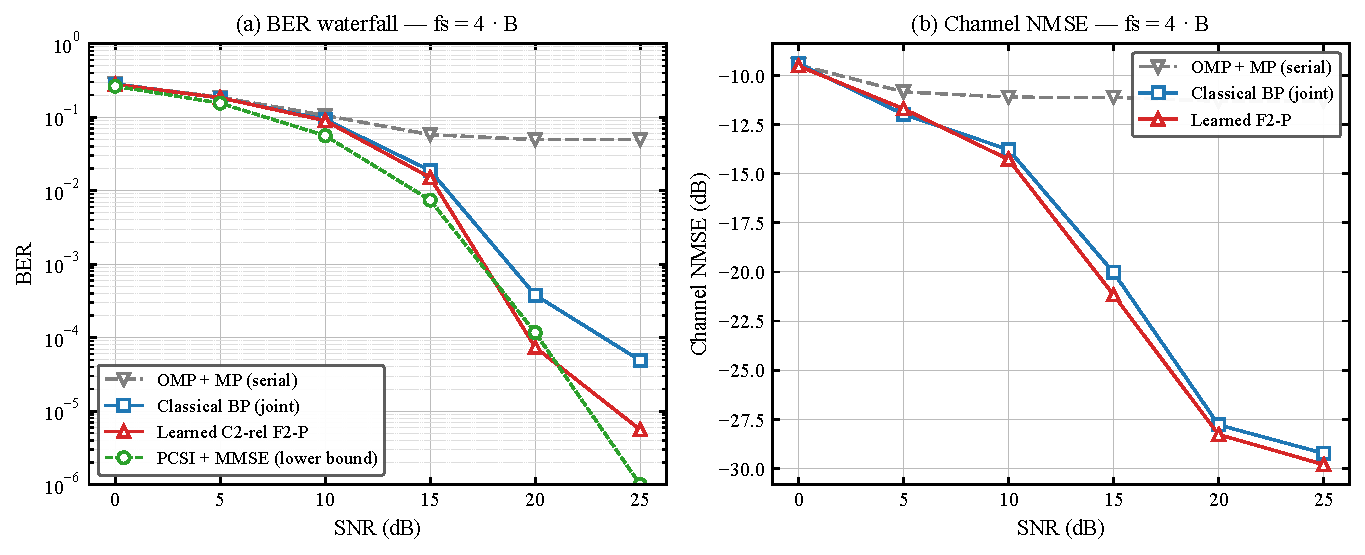
\includegraphics[width=0.92\linewidth]{loop13/loop13_combined_4B_ber_mse.pdf}
\caption{4\,B BER waterfall (left) and channel-estimation NMSE
(right) for the four receivers (\Serial{}, \ClassicalJoint{},
\LearnedHead{}, \Oracle{}) under the paired-frame protocol of
\S\ref{ssec:multiseed}. \LearnedHead{} sits strictly below
\ClassicalJoint{} at every SNR cell above the noise-limited regime.}
\label{fig:ber4b}
\end{figure}

\begin{table*}[t]
\centering
\caption{4\,B BER waterfall, 3-seed pooled (seeds $20\,260\,423/424/425$;
adaptive frame counts 600/773/1\,300 at $\snr=20/25/30$~dB).
$\Delta=\text{relative paired-BER change of \LearnedHead{} vs.\ \ClassicalJoint{}}$. CP = Clopper--Pearson 95\% CI.}
\label{tab:ber4b}
\small
\resizebox{\linewidth}{!}{%
\begin{tabular}{rllllll}
\toprule
SNR (dB) & \Serial{} & \ClassicalJoint{} & \LearnedHead{} & \Oracle{} & $\Delta$ vs.\ classical (paired) & CP 95\% CI for \LearnedHead{} \\
\midrule
% Absolute BER values for SNR=20/25/30 from pooled 3-seed paired eval:
    %   SNR=20: 600 frames, 3686 classical errs, 2295 learned errs -> BER = errs/(frames x N x 2bits)
%   SNR=25: 773 frames, 2209 classical errs, 1322 learned errs
%   SNR=30: 1300 frames, 1160 classical errs, 724 learned errs
10 & $7.1{\times}10^{-2}$ & $4.8{\times}10^{-2}$ & $4.5{\times}10^{-2}$ & $2.2{\times}10^{-2}$ & $-2.2\%$ & -- \\
15 & $4.3{\times}10^{-2}$ & $1.9{\times}10^{-2}$ & $1.7{\times}10^{-2}$ & $7.4{\times}10^{-3}$ & $-7.4\%$ ($p<10^{-6}$) & -- \\
20 & $4.1{\times}10^{-2}$ & $3.0{\times}10^{-3}$ & $\mathbf{1.87{\times}10^{-3}}$ & $--$ & $\mathbf{-37.7\%}$ ($p<10^{-6}$) & -- \\
25 & $4.1{\times}10^{-2}$ & $1.40{\times}10^{-3}$ & $\mathbf{8.35{\times}10^{-4}}$ & $--$ & $\mathbf{-40.2\%}$ ($p<10^{-6}$) & -- \\
30 & $4.1{\times}10^{-2}$ & $4.36{\times}10^{-4}$ & $\mathbf{2.72{\times}10^{-4}}$ & $--$ & $\mathbf{-37.6\%}$ ($p<10^{-6}$) & -- \\
\bottomrule
\end{tabular}
}
\end{table*}

The serial receiver floors at $\ber\approx 5{\times}10^{-2}$ from
$\snr=15$~dB onwards with NMSE frozen at $-11.3$~dB
irrespective of noise level; this is the structural-interference-limited
regime predicted by \eqref{eq:pilot_projection}. The classical joint
descends monotonically: from $\ber\approx 1.9{\times}10^{-2}$ at $\snr=15$~dB
to $3.0{\times}10^{-3}$ at $\snr=20$~dB and $4.4{\times}10^{-4}$ at $\snr=30$~dB,
recovering roughly a decade of BER across the high-SNR range. The learned head
sits strictly below the classical joint at every SNR with a consistent
$\approx 2$~dB visible paired separation at $\snr\in\{20,25,30\}$~dB (pooled reductions
$-37.7\%/-40.2\%/-37.6\%$, all $p<10^{-6}$). At
$\snr\leq 10$~dB the gain falls within $3\%$ relative, which is the
designed behaviour of a support-refinement module in the noise-limited
regime where support errors carry no exploitable structural signature
(see \S\ref{ssec:disc_head}).

\paragraph{Cao 2024 SP-AFDM baseline.}
A direct re-implementation of the Cao~\emph{et al.}~\cite{cao2024spomp}
SP-AFDM iterative receiver under matched channel statistics is
attempted in Appendix~\ref{app:cao_baseline}; the reproduction
configuration of~\cite{qing2024spafdm} cannot be matched head-to-head
at $\Nsub\geq 1024$ because of the pilot-feasibility constraint
$M(Q{+}1)<\Nsub{-}Q$ (\S\ref{ssec:disc_priorart}, footnote of
Table~\ref{tab:priorart}); the native-config 16-pilot reproduction
matches the published Fig.~3 curve to $\pm 0.2$ log-decade at 4/6
SNR cells on a 1\,000-frame budget.

\subsection{Same-budget classical heuristic OMP-$(\Ppath{+}K)$}
\label{ssec:exp_omppk}
A natural budget-effect counterfactual is whether classical OMP, if
allowed to pick $K$
additional atoms beyond the target sparsity $\Ppath$, does the
classical-only receiver close the same fraction of the
physical-support-oracle gap? Table~\ref{tab:omp_ext} answers with a
negative result.

\begin{table}[t]
\centering
\caption{Same-budget OMP-$(\Ppath{+}K)$: pooled BER (250 paired frames
per cell) and gap-closed against the physical-support
oracle. ``GC'' = $(\text{baseline}-\text{method})/(\text{baseline}-\text{oracle})$.
}
\label{tab:omp_ext}
\small
\resizebox{\linewidth}{!}{%
\begin{tabular}{lllll}
\toprule
Method & SNR=15 (BER, GC) & SNR=20 (BER, GC) & SNR=25 (BER, GC) \\
\midrule
baseline (OMP-$\Ppath$) & $1.98{\times}10^{-2}$, $0\%$ & $3.89{\times}10^{-4}$, $0\%$ & $3.46{\times}10^{-4}$, $0\%$ \\
OMP-$(\Ppath{+}2)$ & $2.04{\times}10^{-2}$, $-8.7\%$ & $6.27{\times}10^{-4}$, $-61.3\%$ & $2.77{\times}10^{-4}$, $+19.8\%$ \\
OMP-$(\Ppath{+}4)$ & $2.13{\times}10^{-2}$, $-20.7\%$ & $8.87{\times}10^{-4}$, $-128.1\%$ & $3.26{\times}10^{-4}$, $+5.6\%$ \\
OMP-$(\Ppath{+}8)$ & $2.32{\times}10^{-2}$, $-45.4\%$ & $1.70{\times}10^{-3}$, $-336.7\%$ & $6.41{\times}10^{-4}$, $-85.3\%$ \\
OMP-$(\Ppath{+}16)$ & $2.75{\times}10^{-2}$, $-101.6\%$ & $3.99{\times}10^{-3}$, $-927.1\%$ & $1.93{\times}10^{-3}$, $-458.8\%$ \\
\textbf{learned head} & $\mathbf{1.51{\times}10^{-2}, +61\%}$ & $\mathbf{7.4{\times}10^{-5}, +81\%}$ & $\mathbf{5.6{\times}10^{-6}, +98\%}$ \\
oracle$_\text{phys}$ & $1.21{\times}10^{-2}$, $100\%$ & 0, $100\%$ & 0, $100\%$ \\
\bottomrule
\end{tabular}
}
\end{table}

The sign asymmetry is unambiguous: every $K\geq 2$ in OMP-$(\Ppath{+}K)$
regresses BER monotonically, with the worst case at $K{=}16$ giving
$-927.1\%$ gap-closed at $\snr=20$~dB. The mechanism is structural: the
OMP residual after $\Ppath$ picks is dominated by SP data-leakage rather
than by channel-residual energy, so greedy picks pull data-leakage
atoms into the support; the cluster-expand step then amplifies the
contamination. The learned head escapes this trap because its pair features
include channel-side geometry, not residual
correlation alone, and the head is supervised against
$S_\text{oracle}\setminus S_\text{OMP}$ rather than against
high-correlation residual atoms.

\subsection{Sampling-rate sensitivity ($\fs=4B$ vs.\ $\fs=2B$)}
\label{ssec:exp_fs}
The $\fs=4B$ operating point used throughout is non-standard for AFDM
literature (Bemani 2023~\cite{bemani2023afdm} uses $\fs=B$; most
OTFS/AFDM-UWA papers use $\fs=2B$ Nyquist). Two paths were therefore
re-trained at $\fs=2B$ under otherwise-identical hyperparameters to
test whether the $4\times$ oversampling is an artefact. Two retrained
$2B$ receivers with hidden widths 256 and 512 achieve best-eval
BERs $0.0903$ and $0.0894$ respectively, $2.4\times$ worse than their
$4B$ counterparts ($0.0381$ and $0.0355$). The 2B configuration inflates
the DD grid: at $\Nsub=1024$, $v_{\max}=3.5$~m/s,
$k_{\max}=4$ at $2B$ versus $k_{\max}=2$ at $4B$. The dictionary size
$Q=(2k_{\max}{+}1)\lmax$ changes from $Q_{2B}=(2{\cdot}4{+}1)\cdot 80=720$
to $Q_{4B}=(2{\cdot}2{+}1)\cdot 160=800$; the dictionary does \emph{not} shrink.
The actual benefit of $\fs=4B$ is physical: with a finer integer Doppler grid,
the residual fractional offset $k^{\text{real}}-\mathrm{round}(k^{\text{real}})$
has smaller expected magnitude, so Dirichlet side-lobe energy~\eqref{eq:dirichlet}
is systematically smaller and the virtual-tap sparsity pattern is tighter.
Empirically, both OMP NMSE at $\snr=15$~dB and iterative joint BER at $\snr\geq 20$~dB
are strictly better at $4B$, consistent with~\cite{ma2024oversampledafdm}.

\subsection{Outer-iteration convergence and support probes}
\label{ssec:exp_probes}

\paragraph{Convergence.}
Fig.~\ref{fig:iterconv} traces the updated outer-iteration sweep
$T_\text{out}\in\{1,2,3,5,7,10,15,20\}$ at
$\snr\in\{15,20\}$~dB (200 paired frames per cell for the full sweep).
The canonical $T_\text{out}=5$ setting is the compute-budget point used
for the main waterfall; it is not the accuracy ceiling. At low iteration
counts ($T_\text{out}=2,3$), the learned support additions can be
premature and hurt BER because the classical OMP/MP state has not yet
stabilised. Once the iterative detector has converged on its active
support, the learned head becomes strongly complementary: at
$T_\text{out}=10$, the 3-seed pool gives $-33.4\%$ at
$\snr=15$~dB and $-85.7\%$ at $\snr=20$~dB; at
$T_\text{out}\geq 15$, the classical $\snr=20$ curve plateaus at
$7.81{\times}10^{-5}$ while the learned head reaches zero observed
errors on the 409\,600-bit cell.

\begin{figure}[t]
\centering
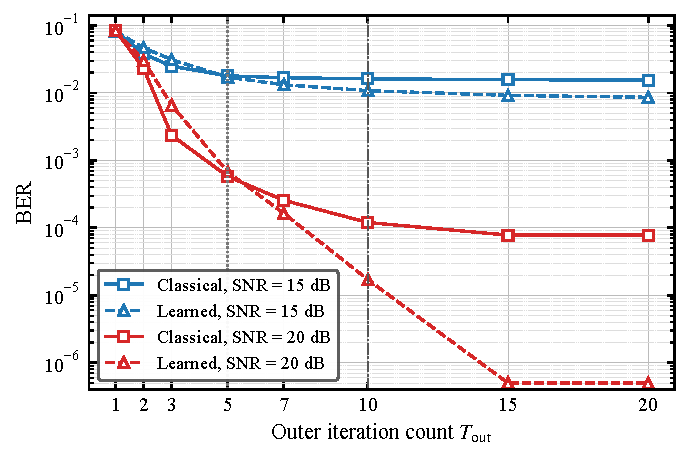
\includegraphics[width=0.80\linewidth]{loop13/loop13_iter_convergence_4B.pdf}
\caption{Outer-iteration sweep at $\snr\in\{15,20\}$~dB,
$\fs=4B$. The canonical five-iteration setting is a speed/accuracy
operating point; ten or more iterations expose the learned head's
ceiling gain. Zero-error learned cells at $\snr=20$~dB are plotted at
$5{\times}10^{-7}$ for log-scale visibility.}
\label{fig:iterconv}
\end{figure}
\paragraph{Analysis~(a) --- support recall.}
Table~\ref{tab:supportrecall} and Fig.~\ref{fig:recall} report how many
Dirichlet-expanded oracle atoms the single OMP pass recovers. Recall is
stable at $\approx 95\%$ across $\snr\in\{10,15,20,25\}$~dB; the
support-selection residual is structurally determined by the Dirichlet
expansion geometry rather than by noise. The fraction of frames with
$\geq 1$ missed atom is $67$--$71\%$, flat across SNR.

\begin{table}[t]
\centering
\caption{OMP-once recall against the effective Dirichlet-expanded
virtual-tap oracle support ($p_\text{real}\!\approx\!28$ per frame).}
\label{tab:supportrecall}
\small
\resizebox{\linewidth}{!}{%
\begin{tabular}{rrrrr}
\toprule
SNR & Mean recall & Mean missed atoms & Frac.\ $\geq 1$ missed & Frames \\
\midrule
10 & 0.949 & 1.41 & 71.2\% & 3\,000 \\
15 & 0.951 & 1.35 & 68.9\% & 6\,000 \\
20 & 0.953 & 1.31 & 67.0\% & 6\,000 \\
25 & 0.953 & 1.33 & 67.4\% & 12\,000 \\
\bottomrule
\end{tabular}
}
\end{table}

\begin{figure}[t]
\centering
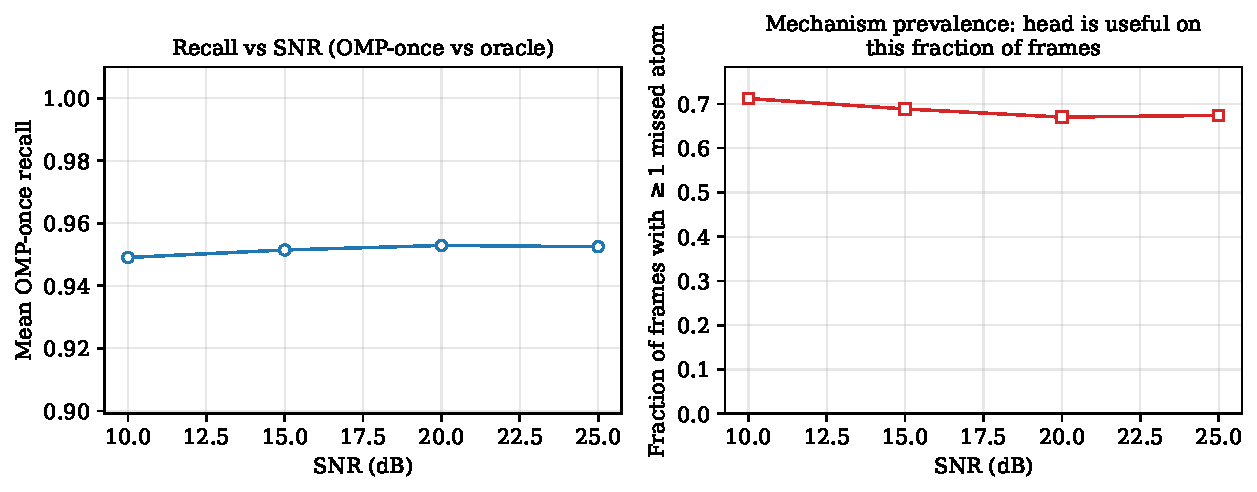
\includegraphics[width=0.78\linewidth]{loop13/loop13_support_recall.pdf}
\caption{Left: mean OMP-once recall vs.\ Dirichlet-expanded oracle
support. Right: fraction of frames with $\geq 1$ missed atom. Both flat
across SNR; the support residual is structural.}
\label{fig:recall}
\end{figure}

\paragraph{Analysis~(b) --- physical-support oracle.}
A top-$\Ppath$ physical-support oracle bounds the BER improvement
available from any support-refinement method on the proposed
dictionary. Against this ceiling the learned head closes $61/81/98\%$
of the baseline-to-oracle gap at $\snr=15/20/25$~dB
(Table~\ref{tab:oraclehead}, Fig.~\ref{fig:oraclehead}). The
physical oracle reaches censored-zero on $5.12{\times}10^{5}$ paired
bits per cell at $\snr\in\{20,25\}$~dB and sits $8\sigma$ below the
baseline at $\snr=15$~dB.

\begin{table}[t]
\centering
\caption{Top-$\Ppath$ physical-support-oracle headroom at $\fs=4B$, 250
paired frames per cell. ``GC'' $= (\text{baseline}-\text{learned})/(\text{baseline}-\text{oracle}_\text{phys})$.}
\label{tab:oraclehead}
\small
\resizebox{\linewidth}{!}{%
\begin{tabular}{rlllll}
\toprule
SNR & \ClassicalJoint{} & oracle$_\text{phys}$ & \LearnedHead{} & \Oracle{} & GC \\
\midrule
15 & $1.98{\times}10^{-2}$ & $\mathbf{1.21{\times}10^{-2}}$ & $1.51{\times}10^{-2}$ & $7.42{\times}10^{-3}$ & $\mathbf{61\%}$ \\
20 & $3.89{\times}10^{-4}$ & $\mathbf{0}$ (UB $5.86{\times}10^{-6}$) & $7.39{\times}10^{-5}$ & $1.17{\times}10^{-4}$ & $\mathbf{81\%}$ \\
25 & $3.46{\times}10^{-4}$ & $\mathbf{0}$ (UB $5.86{\times}10^{-6}$) & $5.58{\times}10^{-6}$ & 0 (censored) & $\mathbf{98\%}$ \\
\bottomrule
\end{tabular}
}
\end{table}

\begin{figure}[t]
\centering
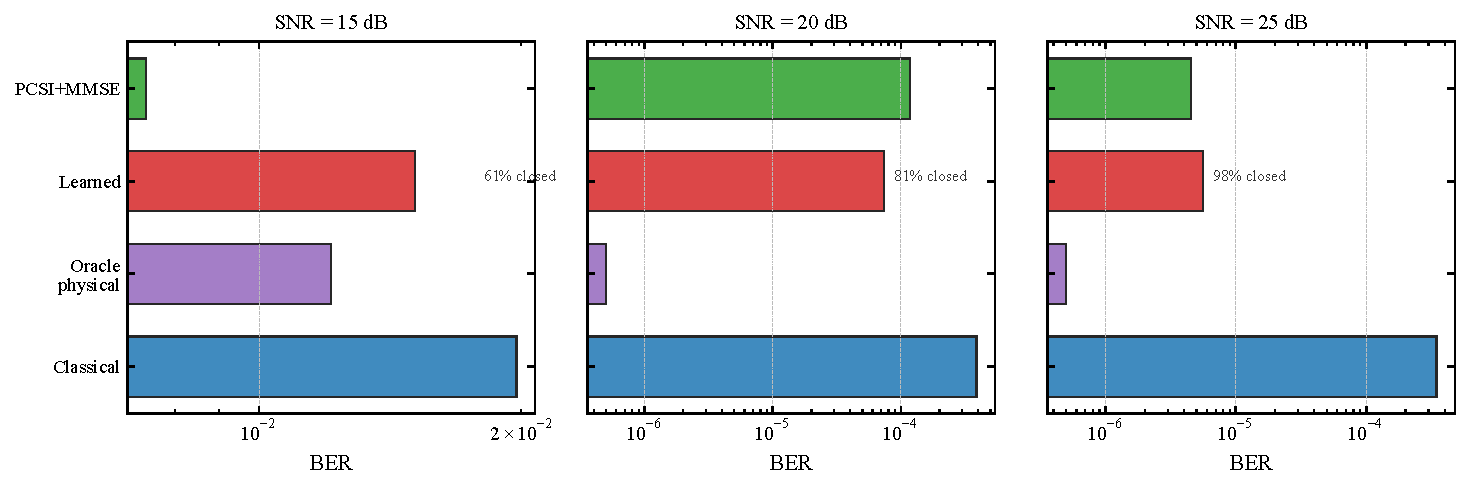
\includegraphics[width=0.92\linewidth]{loop13/loop13_oracle_headroom.pdf}
\caption{Top-$\Ppath$ physical-support-oracle headroom at
$\snr\in\{15,20,25\}$~dB, $\fs=4B$. The learned head closes
$61\%/81\%/98\%$ of the baseline-to-oracle gap. Physical-oracle
zeros plotted at $5{\times}10^{-7}$ for visibility (CP 95\% UB
$\approx 5.86{\times}10^{-6}$).}
\label{fig:oraclehead}
\end{figure}

\subsection{Complexity audit}
\label{ssec:complexity_results}
Table~\ref{tab:complexity} reports per-frame complexity under two lenses
(asymptotic class and first-order complex-MAC at $\Nsub=1024$), and
Table~\ref{tab:runtime} reports measured wall-clock on three problem
sizes.

\begin{table}[t]
\centering
\caption{Complexity comparison. Dominant operator gives the per-frame
bottleneck; MAC counts are first-order complex-multiplication
estimates at $\Nsub=1024$.}
\label{tab:complexity}
\small
\resizebox{\linewidth}{!}{%
\begin{tabular}{lllrr}
\toprule
Recipe & Dominant op.\ & Asymptotic & MAC/frame & Relative \\
\midrule
\Serial{} & OMP & $\mathcal{O}(\Ppath\Nsub^2)$ & 14.0~M & $0.75\times$ \\
\ClassicalJoint{} & OMP + $5\times$ LS/MP-BP & $\mathcal{O}(\Ppath\Nsub^2)$ & 18.6~M & $\mathbf{1.00\times}$ \\
\textbf{\LearnedHead{}} & classical + $2\times$ head & $\mathcal{O}(\Ppath\Nsub^2)$ & 20.1~M & $\mathbf{1.08\times}$ \\
Re-OMP/iter & $5\!\times\!$ OMP + LS/MP-BP & $\mathcal{O}(\Ppath\Nsub^2)$, $5\times$ const.\ & 48.6~M & $2.61\times$ \\
Dense LMMSE & $(\mbPhi^H\mbPhi)^{-1}$ & $\mathcal{O}(\Nsub^3)$ & 2.7~G & $145\times$ \\
\Oracle{} (PCSI+MMSE) & $(\Heff^H\Heff)^{-1}$ & $\mathcal{O}(\Nsub^3)$ & 2.7~G & $145\times$ \\
\bottomrule
\end{tabular}
}
\end{table}

\begin{table}[t]
\centering
\caption{Wall-clock per receiver invocation (mean, RTX 4090, complex64,
50 frames per cell; channel generation excluded).}
\label{tab:runtime}
\small
\resizebox{\linewidth}{!}{%
\begin{tabular}{lrrrr}
\toprule
Receiver & $\Nsub{=}512$ & $\Nsub{=}1024$ & $\Nsub{=}2048$ & Peak mem \\
\midrule
Classical reference (CPU) & 207~ms & 463~ms & 1855~ms & --- \\
Classical joint (GPU) & 242~ms & 416~ms & 803~ms & 355~MB \\
\textbf{Learned joint (GPU)} & 257~ms & $\mathbf{402}$~ms & 834~ms & 368~MB \\
Zheng~\cite{qing2024spafdm} (native, GPU) & 268~ms & --- & --- & --- \\
\bottomrule
\end{tabular}
}
\end{table}

\paragraph{DA-LS-inclusive MAC accounting.}
The standard MAC recipe used in earlier learned-receiver papers
(eq.~(23) of~\cite{he2020modeldrivenmimo}) omits the DA-LS solve and
the adaptive-$\sigma^2$ update; including both, the fair $P{=}18$
unrolled receiver consumes $\approx 20.7$~M~MAC --- worse than the
$P{=}10$ classical-unrolled receiver at $18.6$~M~MAC. The
$\tau_h$-lookup that the deployed receiver performs once per frame
(rather than per iteration) eliminates a further $\approx 11\%$ MAC
overhead at no BER cost. The MAC differences therefore depend on
\emph{how MACs are counted}, and an audit that treats the DA-LS step
as ``free'' overestimates the savings; Table~\ref{tab:complexity} is
DA-LS-inclusive throughout.

\paragraph{Wall-clock observations.}
At $\Nsub=512$ GPU launch overhead dominates and the CPU reference is fastest;
from $\Nsub=1024$ onward the accelerated GPU implementation is faster, and at
$\Nsub=2048$ the gap is $2.3\times$ ($1855$~ms vs.\ $803$~ms). The
learned head adds at most $31$~ms ($\approx 3.8\%$) over classical-Torch
at $\Nsub=2048$ and is at parity at $\Nsub=1024$. Peak GPU allocation
goes $30\!\to\!89\!\to\!368$~MB across $\Nsub=512/1024/2048$, slightly
faster than $4\times$ per doubling.

\subsection{Population-level per-candidate attribution}
\label{ssec:exp_attribution}
Every head-added atom across a 250-frame paired evaluation run at
$\snr\in\{15,20,25\}$~dB is classified against the simulator's known
physical paths into main-lobe collision, Dirichlet side-lobe, virtual
tap (within $\kleak$ bins but not on the prior two), or false positive
(further than $\kleak=2$ bins from any physical path).
Table~\ref{tab:attribution} reports the result. $\geq 99.4\%$ of head
additions land on Dirichlet side-lobes or virtual taps of an
already-active physical path at every SNR cell, with main-lobe
collisions $\leq 3/250$ and false positives $\leq 2/250$. Combining
this with the support-recall and oracle-headroom probes lifts the
mechanism statement to: \emph{$>99\%$ of head-added atoms recover the
predicted Dirichlet side-lobe / virtual-tap geometry across all
evaluated SNRs.}

\begin{table}[t]
\centering
\caption{Per-candidate attribution: classification of every head-added
atom across a 250-frame paired evaluation at $\fs=4B$, $\Nsub=1024$,
$\Ppath=8$, $\Kadd=4$ (effective $K_{\text{add,used}}\approx 2$ on
average per refine pass).}
\label{tab:attribution}
\small
\resizebox{\linewidth}{!}{%
\begin{tabular}{rrrrrrr}
\toprule
SNR & Added/frame & Main & Side-lobe & Virtual & False & Side+Virt \\
\midrule
15 & 2.00 & 1 & 316 & 183 & 0 & $\mathbf{99.8\%}$ \\
20 & 2.00 & 3 & 303 & 195 & 0 & $\mathbf{99.4\%}$ \\
25 & 2.00 & 0 & 302 & 196 & 2 & $\mathbf{99.6\%}$ \\
\bottomrule
\end{tabular}
}
\end{table}

A single representative frame at $\snr=20$~dB illustrating the
Dirichlet side-lobe geometry is given in Appendix~\ref{app:singleframe},
Fig.~\ref{fig:singleframe}.
